\documentclass{article}

\usepackage[T2A]{fontenc}
\usepackage[utf8]{inputenc} 
\usepackage[english,russian]{babel} 
\usepackage{graphicx} 
\usepackage{amsmath}
\usepackage{amssymb}
\usepackage{cancel}
\usepackage{amsfonts}
\usepackage{titlesec}
\usepackage{titling} 
\usepackage{geometry}
\usepackage{pgfplots}
\pgfplotsset{compat=1.9}


\titleformat{\section}
{\normalfont\Large\bfseries}{\arabic{section}}{1em}{}
\titleformat{\subsection}
{\normalfont\large\bfseries}{}{1em}{}


\setlength{\droptitle}{-3em} 
\title{\vspace{-1cm}ИДЗ №1}
\author{Винницкая Дина Сергеевна}
\date{Группа: Б9122-02-03-01сцт}

\geometry{a4paper, margin=2cm}

\begin{document}
	
	\maketitle

	\section{Найти все значения корня:$\sqrt[4]{\frac{-1 + i\sqrt{3}}{2}}$}
	\subsection{Решение:}
        $$\sqrt[4]{\frac{-1 + i\sqrt{3}}{2}} \implies \sqrt[4]{-1 + i\sqrt{3}}  $$\\
        Необходимо перейти к тригонометрической форме: \\
        $$x = Re(z) = -1; \quad y = Im(z) =  \sqrt{3} $$
        $$arg(z) = \psi = \pi - \arctan(\frac{y}{|x|}) \implies z - \psi - \pi - \arctan(\frac{\sqrt{3}}{|-1|}) = \pi - \frac{\pi}{3} = \frac{2\pi}{3}$$
        Тригонометрическая форма комплексного числа: \\
        $$z = \cos(\frac{2\pi}{3}) + i\sin(\frac{2\pi}{3})$$ 
        $$z_k = \sqrt[4]{|z|} =  \sqrt[4]{|z|} \cos(\frac{\psi 2 \pi k}{4}) + i\sin(\frac{\psi 2 \pi k}{4}),\quad k = 0,1,2,3 ... $$ 
        $$w_0 = \cos(\frac{\pi}{6}) + i\sin(\frac{\pi}{6})$$
        $$w_1 = \cos(\frac{2\pi}{3}) + i\sin(\frac{2\pi}{3})$$
        $$w_2 = \cos(\frac{7\pi}{6}) + i\sin(\frac{7\pi}{6})$$
        $$w_3 = \cos(\frac{5\pi}{3}) + i\sin(\frac{5\pi}{3})$$

        \section{Представить в алгебраической форме: $\cos(\frac{\pi}{2}- i)$}
        \subsection{Решение:}
        Воспользуемся тригонометрической формулой: \\
        $$\cos(\alpha \pm \beta) = \cos(\alpha) \cos(\beta) \mp \sin(\alpha)\sin(\beta)$$ 
        $$\cos(\frac{\pi}{2}- i) = \cos(\frac{\pi}{2}) \cos(i) + \sin(\frac{\pi}{2}) \sin(i) = 0 \ch(1) + i\sh(1) = i\sh(1)$$
        
	\subsection{Ответ:$\quad i\sh(1)$}

        \section{Представить в алгебраической форме: $\arccos(-3i)$}
        \subsection{Решение:}
        $$\arccos(-3i) = \theta \implies \cos(\theta) = -3i$$ 
        $$\theta: [\theta = \arccos(-3i) = \pi + i \ln(3 + \sqrt{3^2 - 1})]$$
        $$\arccos(-3i) = \pi + i \ln(3 + \sqrt{8})$$
	
	\subsection{Ответ:$\quad \pi + i \ln(3 + \sqrt{8})$}

        \section{Представить в алгебраической форме: $(2 + i)^{-3i}$}
	\subsection{Решение:}
	$$(2 + i)^{-3i} = e^{-3i\ln(2 + i)}$$
        $$\ln(2 + i) = \ln{|2 + i|} + iArg(2 + i) = \ln{\sqrt{5}} + i(\arctan{\frac{1}{2}} + 2\pi n),\quad n \in \mathbb{Z} $$ 
        Таким образом, получаем: \\
         $$(2 + i)^{-3i} = e^{-3i(\ln{\sqrt{5}} + i(\arctan{\frac{1}{2}} + 2\pi n)} = e^{3(\arctan{\frac{1}{2}} +  2\pi n)} (\cos(3\ln{\sqrt{5}}) + i\sin(3\ln{\sqrt{5}})$$
	\subsection{Ответ:$\quad e^{3(\arctan{\frac{1}{2}} +  2\pi n)} (\cos(3\ln{\sqrt{5}}) + i\sin(3\ln{\sqrt{5}})$}

        \section{Представить в алгебраической форме: $\text{Ln}(2+2\sqrt{3}i)$}
	\subsection{Решение:}
	\[\text{Ln}(2+2\sqrt{3}i) = \ln|2 + 2\sqrt{3}i| + i\text{Arg}(2+2\sqrt{3}i) = \ln 4 + i\left(\frac{\pi}{3} + 2\pi k\right), k \in \mathbb{Z}\]
	\subsection{Ответ:$\quad\ln 4 + i\left(\frac{\pi}{3} + 2\pi k\right), k \in \mathbb{Z}$}
 
        \section{Вычертить область, заданную неравествами: $\\D = \{z : 1 < z\bar{z} < 2, Re(z) > 0, 0 \le Im(z) \le 1 \}$}
	\subsection{Ответ:}
        \begin{figure}[h]
            \centering
            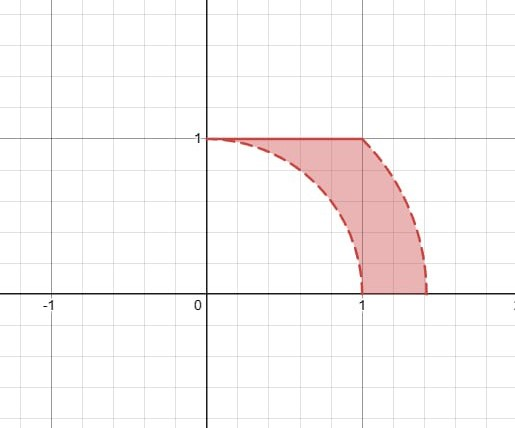
\includegraphics[width=0.5\textwidth]{gr_1.jpg}
            \label{fig:my_label}
        \end{figure}

        \section{Определить вид пути и в случае, когда он проходит через точку $\infty$, исследовать его поведение в этой точке: $z = 3\tan{t}+i4\sec{t}$}
	\subsection{Решение:}
         Наименьший общий период функций $\sec$ и $\tan$ равен $2\pi$ $\implies$ достаточно построить кривую для: $$t \in (-\frac{\pi}{2};\quad \frac{\pi}{2})\cup t \in (\frac{\pi}{2};\quad \frac{3\pi}{2})$$
        Параметрические уравнения кривой, которую необходимо найти имеют вид:\\
        \[
        \begin{cases}
        x = 3\tan{t} \\
        y = 4\sec{t}
        \end{cases}
        \]
        Исключим параметр t:\\
        \[
        \begin{aligned}
        & \frac{x}{3} = \tan{t} & \quad & \frac{y}{4} = \sec{t} \\
        & \frac{x^2}{9} = \tan^2{t} + 1 - 1 & \quad & \frac{y^2}{6} = \sec^2{t} \\
        & \frac{x^2}{9} = \frac{1}{\cos^2{t} - 1} & \quad & \frac{y^2}{6} = \frac{1}{\cos^2{t}} \\
        \end{aligned}
        \]
        $\implies \quad \frac{x^2}{9} = \frac{y^2}{16} - 1  \quad \frac{x^2}{9} - \frac{y^2}{16} = -1$ - каноническое уравнение гиперболы $\quad\quad \frac{x}{3} \mp \frac{y}{4} = 0$ - асимптоты \\
         \begin{figure}[h]
            \centering
            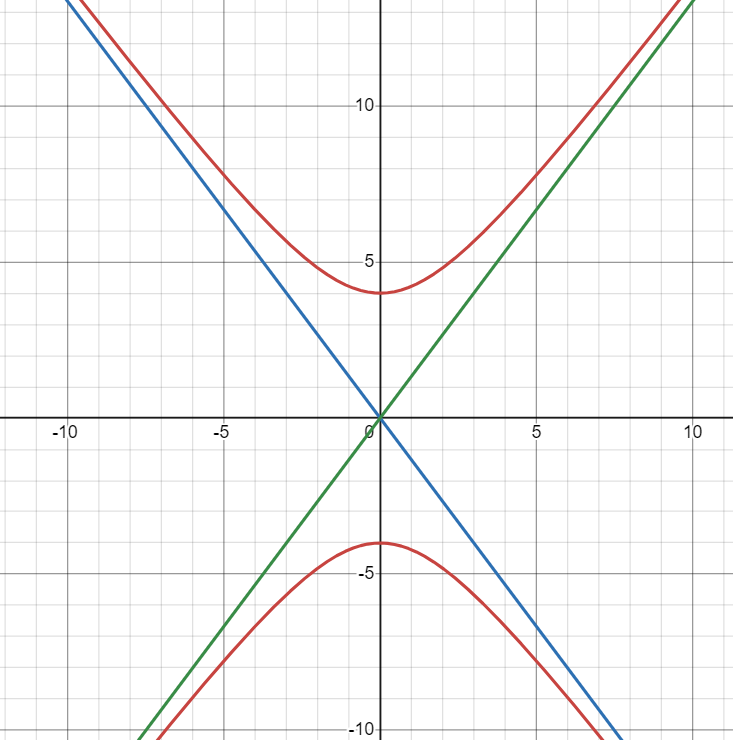
\includegraphics[width=0.5\textwidth]{gr_2.png}
            \label{fig:my_label}
        \end{figure}
        $$t \rightarrow  -\frac{\pi}{2} + 0, \quad x \rightarrow -\infty \quad y \rightarrow +\infty$$
        $$t \rightarrow  \frac{\pi}{2} - 0, \quad x \rightarrow +\infty \quad y \rightarrow +\infty$$
        $$t \rightarrow  \frac{\pi}{2} + 0, \quad x \rightarrow -\infty \quad y \rightarrow -\infty$$
        $$t \rightarrow  \frac{3\pi}{2} -  0, \quad x \rightarrow +\infty \quad y \rightarrow -\infty$$

         \section{Восстановить голоморфную в окрестности точки $z_0$ функцию $f(z)$ по известной действительной части $u(x,y)$ или мнимой $v(x,y)$ и начальному значению $f(z_0)$: $-2xy-2y, \ f(0) = i$}
	\subsection{Решение:}
        \begin{equation}
        \left\{
        \begin{array}{ll}
        \frac{du}{dx} = -2y & \quad\quad \frac{d^2u}{dx^2} = 0 \\
        \frac{du}{dy} = -2x - 2 & \quad\quad \frac{d^2u}{dy^2} = 0
        \end{array}
        \right.
        \end{equation}
        $$\implies \triangle u = 0$$
        Удовлетворяет уравнению Лапласа \\
         \begin{equation}
        \left\{
        \begin{array}{ll}
        \frac{du}{dx} = \frac{dv}{dy} \\
        \frac{du}{dy} = -\frac{dv}{dx}
        \end{array}
        \right.
        \end{equation}
        Условие Коши-Римана\\
        \begin{equation}
        \left\{
        \begin{array}{ll}
        \frac{du}{dx} = \frac{dv}{dy} \quad \implies v = x^2 + 2x + \phi{y} \\
        \frac{du}{dy} = -\frac{dv}{dx} \quad \implies \phi'{(y)}
        \end{array}
        \right.
        \end{equation}
        $$\phi(y) = -y^2 + C$$
        $$v(x, y) = x^2 + 2x - y^2 + C$$
        $$f(x, y) = -2xy - 2y + i(x^2 + 2x - y^2 + C$$
        Голоморфная функция \\
        $$f(z) = u(x, y) + iv(x, y) = -2xy - 2y + i(x^2 + 2x - y^2 + C) = -2xy - 2y + ix^2 + 2ix - iy^2 + C \cdot i =$$
        $$= (ix^2 - iy^2 - 2xy) + (-2y + 2ix) + C \cdot i \circeq$$
        $$z^2 \cdot i = ix^2 - iy^2 - 2xy$$
        $$2z \cdot i = -2y + 2ix$$
        $$\circeq z^2 \cdot i + 2z \cdot i + C \cdot i$$
        $$f(0) = i = i \cdot C \quad\quad C = 1$$
        $$f(x) = z^2 \cdot i + 2z \cdot i + i = i(z^2 + 2z + 1)$$
        \subsection{Ответ:$\quad f(x) = i(z^2 + 2z + 1)$}

        \section{Вычислить интеграл от функции комплексной переменной по данному пути: $\int_{ABC} z\bar{z}dz; \ AB = \{z: |z| = 1,\quad Re(z) \ge 0,\quad Im(z) \ge 0  \}\quad \textbf{BC - отрезок прямой}$}
	\subsection{Решение:}
        $$y = \{0 < x < 1\} $$
        \begin{figure}[h]
            \centering
            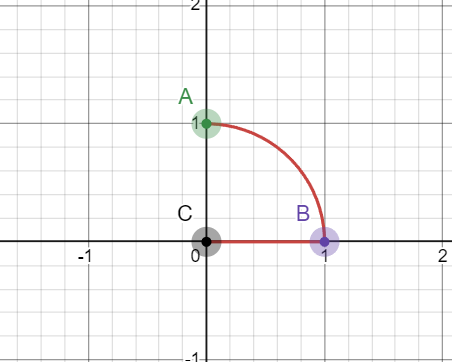
\includegraphics[width=0.5\textwidth]{gr_3.png}
            \label{fig:my_label}
        \end{figure}
        $A = (0, 1) \quad B = (1, 0) \quad C = (0, 0)$
        $$I = \int_{ABC} z\bar{z}dz = \int_{ABC} (x + iy)(x + iy)dz = \int_{ABC} (x^2 + y^2)dz $$
        $$f(x + iy) = x^2 + y^2 \implies \textbf{мнимая часть функции равна 0}$$
        $$\implies \text{из условия Коши-Римана выполняться не будет, следовательно применяем параметризацию}$$
        $$\int_{ABC} = -\int_{CBA} = -\int_{CB} - \int_{AB} - \textbf{аддитивность области}$$
        $CB:\quad (t;0)\quad 0 \le t \le 1$ \\
        $BA:\quad (\cos{t};sin{t})\quad 0 \le t \le \frac{\pi}{2}$
        $$I =-\int_{CB} (x^2 + y^2)dz - \int_{AB}(x^2 + y^2)dz = -\int_{0}^{1} t^2 \, dt - \int_{0}^{\frac{\pi}{2}} (\cos^2{t} + sin^2{t}) d(\cos{t} + i\sin{t})$$
        $$I = -\frac{1}{3} - \int_{0}^{\frac{\pi}{2}} d(e^{it}) = -\frac{1}{3} - (e{\frac{i\pi}{2}} - e^0) = \frac{2}{3} - i$$
        \subsection{Ответ:$\quad \frac{2}{3} - i$}

        \section{Найти радиус сходимости степенного ряда: $\sum\limits_{n=1}^{\infty}(1 + i)^n \cdot \sin{n} \cdot z^n$}
	\subsection{Решение:}
        $$\implies R = \frac{1}{p}; \quad p = \lim_{{k \to \infty}}  \sqrt[n]{|C_n|}
        $$
        $$\sum\limits_{k=0}^{\infty}C_n \cdot (z-z_0)^n \implies C_n = (1 + i)^n \cdot \sin{n}, \quad |C_n| = 2^{\frac{n}{2}} |\sin{n}|$$
        $$\sqrt[n]{|C_n|} = \sqrt{2} \cdot \sqrt[n]{|\sin{n}|} \le \sqrt{2}$$
        $$\sin{n} \le 1$$

         \begin{figure}[h]
            \centering
            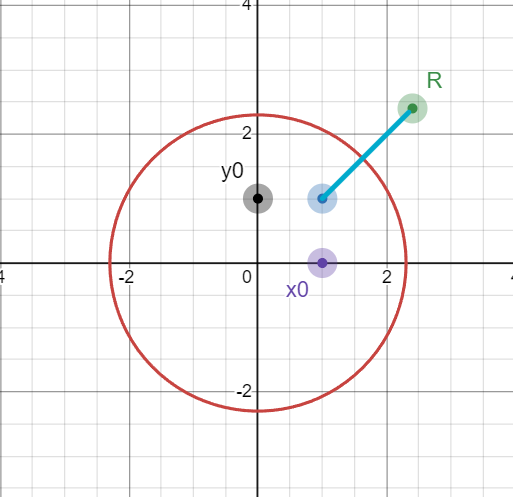
\includegraphics[width=0.5\textwidth]{rg_4.png}
            \label{fig:my_label}
        \end{figure}
        
        $$\exists \quad n_k  \xrightarrow{n \rightarrow \infty} \infty \cdot \sin{n + 1} \rightarrow 0 \neq 0$$
        $$\sqrt[n_k]{|\sin{|n_k|}} \le 1, \quad k > \mathbb{N}$$
        $$|\sin{n_k}|  \rightarrow |\alpha| \neq 0  $$
        $$\sqrt{2} = \lim_{{k \to \infty}} \sqrt{2} \cdot \sqrt[n_k]{\frac{|\alpha|}{2}} = \lim_{{n \to \infty}} \sqrt{2} \sqrt[n]{|\sin{n}|} \le \sqrt{2}$$
        
        \section{Найти лорановские разложения данной функции в 0 и в $\infty$: $f(z) = \frac{3z+36}{18z^2 + 3z^3 -  z^4}$}
	\subsection{Решение:}
        Чтобы найти нужное разложение, предварительно разложим нашу функцию на простые дроби. Для этого найдём все корни знаменателя: 
        $$-z^4 + 3z^3 + 18z^2 = 0 \quad \Leftrightarrow \quad z^2(z^2 - 3z - 18) = 0$$
        $$
        z_1 = z_2 = 0 \quad x_3 = -3 \quad x_4 = 6
        $$
        Таким образом, $-z^4 + 3z^3 + 18z^2 = z^2(z^2 - 3z - 18)$ поэтому разложение
        нашей функции на простые дроби должно иметь вид: 
        $$\frac{3z + 36}{-z^4 + 3z^3 + 18z^2} = \frac{3z + 36}{z^2(z^2 - 3z - 18)} = \frac{3z + 36}{z^2(z + 3)(z - 6)} = \frac{A}{z} + \frac{B}{z^2} + \frac{C}{z + 3} + \frac{D}{z - 6}$$
        Коэффициенты A, B, C, D можно найти как обычно, приводя к общему знаменателю справа и приравнивая коэффициенты при одинаковых степенях z слева и справа. Но B, C и D можно найти проще. Для нахождения B: умножаем обе части равенства на $z^2$ и в результат подставляем $z = 0$: 
        $$\left. \frac{3z + 36}{(z + 3)(z - 6)} \right|_{z = 0} = (Az + B + \frac{Cz^2}{z + 3} + \frac{Dz^2}{z - 6}) \implies B = -2 $$
        $$\left. \frac{3z + 36}{z^2(z - 6)} \right|_{z = -3} = (\frac{A(z + 3)}{z}+ \frac{B(z + 3)}{z^2} + C + \frac{D(z + 3)}{z - 6} ) \implies C = -\frac{1}{3} $$
        $$\left. \frac{3z + 36}{z^2(z + 3)} \right|_{z = 6} = (\frac{A(z - 6)}{z}+ \frac{B(z - 6)}{z^2} + \frac{C(z - 6)}{z + 3} + D) \implies D = \frac{1}{6} $$
        $$\frac{3z + 36}{z^2(z + 3)(z - 6)} = \frac{A}{z} - \frac{2}{z^2} - \frac{1}{3(z + 3)} + \frac{1}{6(z - 6)} \implies A = \frac{1}{6}$$
        $$\implies \quad \frac{3z + 36}{z^2(z + 3)(z - 6)} = \frac{1}{6z} - \frac{2}{z^2} - \frac{1}{3(z + 3)} + \frac{1}{6(z - 6)}$$
        Нам надо найти разложение нашей функции в окрестностях нуля и бесконечности. Оба эти разложения по степеням z. Первые два слагаемые — это уже суммы степеней z. Поэтому остаётся разложить в ряды Лорана только последние слагаемые $\frac{1}{3(z + 3)}$ и  $\frac{1}{6(z - 6)}$.
        Разложим $\frac{1}{3(z + 3)}$ в окрестности нуля. Очевидно, эта функция голоморфна в круге $|z| < 3$. Поэтому её ряд Лорана в этом круге совпадёт с рядом Тейлора (с кругом сходимости $|z| < 3$):
        $$\frac{1}{3(z + 3)} = \frac{1}{3^n} \cdot \frac{1}{(1 + \frac{z}{3})} = \frac{1}{3^2} \cdot \sum\limits_{n=0}^{\infty} \quad (-1)^n (\frac{z}{3})^n = \sum\limits_{n=0}^{\infty} \quad \frac{(-1)^n}{3^{n + 2}} \cdot z^n$$ 
        Аналогично находим разложение $\frac{1}{6(z - 6)}$ в окрестности 0. Замечаем, что функция голоморфна в круге  $|z| < 6$, поэтому
        $$\frac{1}{6(z - 6)} = \frac{1}{6^n} \cdot \frac{1}{(1 + \frac{z}{3})} = \frac{1}{6^2} \cdot \sum\limits_{n=0}^{\infty} \quad (-1)^n (\frac{z}{6})^n = \sum\limits_{n=0}^{\infty} \quad \frac{(-1)^n}{6^{n + 2}} \cdot z^n$$ 
        Оба полученных разложения справедливы в меньшем круге $|z| < 6$. Поэтому в этом круге имеет место равенство
        $$\quad \frac{3z + 36}{z^2(z + 3)(z - 6)} = \frac{1}{6z} - \frac{2}{z^2} - \frac{1}{3(z + 3)} + \frac{1}{6(z - 6)} = \frac{1}{6z} - \frac{2}{z^2} - \sum\limits_{n=0}^{\infty} \quad \frac{(-1)^n}{3^{n + 2}} \cdot z^n + \sum\limits_{n=0}^{\infty} \quad \frac{(-1)^n}{6^{n + 2}} \cdot z^n $$
        $$\frac{1}{6z} - \frac{2}{z^2} - \sum\limits_{n=0}^{\infty} \quad (\frac{(-1)^n}{3^{n + 2}} + \frac{(-1)^n}{6^{n + 2}}) \cdot z^n \quad\quad 0 < z < 6$$
        Отсюда видим, что в кольце $0 < z < 6$ разложение в ряд Лорана имеет вид:
        $$\frac{3z + 36}{z^2(z + 3)(z - 6)} = \frac{1}{6z} - \frac{2}{z^2} - \sum\limits_{n=0}^{\infty} \quad (\frac{(-1)^n}{3^{n + 2}} + \frac{(-1)^n}{6^{n + 2}})  = \sum\limits_{n=-\infty}^{\infty} C_n z^n  $$
        \begin{equation}
        \left\{
        \begin{array}{ll}
        0, \quad n \le -3\\
        -2, \quad n = 2\\
        -\frac{1}{3} \quad n = -1 \\
        \frac{(-1)^n}{3^{n + 2}} + \frac{1}{6^{n + 2}} \quad n \ge 0
        \end{array}
        \right.
        \end{equation}
        Разложим теперь $\frac{1}{(1 + \frac{z}{3})}$ в окрестности $\infty$. Очевидно, эта функция голоморфна в кольце $|z| > 3$. Поэтому преобразуем её так:
        $$\frac{1}{(1 + \frac{z}{3})} = \frac{1}{3z} \cdot \frac{1}{(1 + \frac{3}{z}} \quad\quad |z| > 3 \quad |\frac{3}{z}| < 1 $$
        $$\frac{1}{1 + \frac{3}{z}} = \sum\limits_{n=0}^{\infty} \quad (-1)^n (\frac{3}{z})^n$$
        $$\frac{1}{3(z + 3)} = \frac{1}{3z} \cdot \frac{1}{(1 + \frac{3}{z}} = \frac{1}{3z} \cdot \sum\limits_{n=0}^{\infty} \quad (-1)^n (\frac{3}{z})^n = \sum\limits_{n=0}^{\infty} \quad (-1)^n \cdot \frac{3^{n - 1}}{z^{n + 1}} = n + 1 = n' = \sum\limits_{n=0}^{\infty} \quad \sum\limits_{n' = -\infty}^{-1} \quad \frac{(-1)^{n' + 1}}{3^{n'+ 2}} \cdot z^{n'}$$

         Разложим теперь $\frac{1}{(1 + \frac{z}{3})}$ в окрестности $\infty$. Очевидно, эта функция голоморфна в кольце $|z| > 3$. Поэтому преобразуем её так:
        $$\frac{1}{(1 + \frac{z}{3})} = \frac{1}{3z} \cdot \frac{1}{(1 + \frac{3}{z}} \quad\quad |z| > 3 \quad |\frac{3}{z}| < 1 $$
        $$\frac{1}{1 + \frac{6}{z}} = \frac{1}{6z} \cdot \frac{1}{\left(1 - \frac{6}{z}\right)} = \frac{1}{6z} \sum\limits_{n=0}^{\infty} \left(\frac{6}{z}\right)^n = \sum\limits_{n=0}^{\infty} \frac{6^{n}}{z^{n + 1}} = \sum\limits_{n' = -\infty}^{-1} \frac{1}{6^{n + 2}} \cdot z^{n'} $$
        Оба полученных разложения справедливы в кольце $|z| > 6$. Поэтому в этом кольце имеет место равенство
        $$\frac{3z + 36}{z^2(z + 3)(z - 6)} = \frac{1}{6z} - \frac{2}{z^2} - \sum\limits_{n=-\infty}^{-1} \quad (\frac{(-1)^n}{3^{n + 2}} + \frac{1}{6^{n + 2}})$$

        
        \section{Найти все лорановское разложение данной функции по степеням $z - z_0$: $f(z) = \frac{z - 2}{(z + 1) \cdot (z + 3)},\  z_0 = -2 -i $}
	\subsection{Решение:}
        $$\frac{1}{z \cdot (1 + \frac{1}{z})} = \frac{1}{z} \cdot (\sum\limits_{n=0}^{\infty} \quad (-1)^n \cdot (\frac{1}{z})^n) = \sum\limits_{n=0}^{\infty} \quad (-1)^n \cdot \frac{1}{z^{n + 1}} = \sum\limits_{n=0}^{\infty} \quad (-1)^{n + 1} \cdot z^n$$
        
	$$\frac{1}{z} = \sum\limits_{k=-\infty}^{-1} \quad (-1)^{n + 1} \cdot z^n, \quad \quad |z| > 0$$
        $$\frac{z -2 }{(z + 1)(z - 3)} = \frac{A}{(z + 1)} + \frac{B}{(z - 3)} = \frac{1}{4} = (\frac{3}{(z + 1)} + \frac{1}{(z - 3)})$$
        $$f(z) = \sum\limits_{n=0}^{\infty} \quad \frac{1}{4} (\frac{3\cdot(-1)^n}{(1 + z_0)^{n + 1}} + \frac{(-1)^n}{(z_0 - 3)^{n + 1}} \cdot (z - z_0)^n$$
	$$f(z) = \sum\limits_{n=0}^{\infty} \frac{3}{4} (\frac{(-1)^{n + 1}}{(1 + z_0)^{n + 1}} \cdot (z - z_0)^n + \sum\limits_{n=0}^{\infty} \quad \frac{(-1)^{n + 1}}{4(z_0 - 3)^{n + 1}} \cdot (z - z_0)^n$$

        $$I: \quad \{z: \quad 0 < |z - z_0| < \sqrt{2}$$
        $$II: \quad \{z: \quad \sqrt{2} < |z - z_0| < \sqrt{26}$$
        $$III: \quad \{z: \quad \sqrt{26} < |z - z_0| < \infty$$
        $$VI: \quad \{z: \quad 0 < |z - z_0| > \sqrt{26}$$

        $$\frac{1}{1 + z} = \frac{1}{1 + z_0 + z - z_0} = \frac{1}{(1 + z_0) (1 + \frac{z - z_0}{1 + z_0}} = \frac{1}{(1 + z_0)}\cdot \sum\limits_{n=0}^{\infty} \quad (-1)^n \cdot (\frac{z - z_0}{1 + z_0)})^n = \sum\limits_{n=0}^{\infty} \quad \frac{(-1)^n}{(1 +  z_0)^{n + 1}} \cdot (z - z_0)^n $$
        $$I: \quad \quad \frac{1}{1 + z} = \sum\limits_{n=0}^{\infty} \quad \frac{(-1)^n}{(1 + z_0)^n} \cdot (z - z_0)^n = \frac{1}{z - z_0} \cdot \frac{1}{\frac{1 + f_0}{z - z_0}}$$
        $$\frac{1}{z - z_0} \cdot \sum\limits_{n=0}^{\infty} \quad (-1)^n (\frac{1 + z_0}{z - z_0})^n = \sum\limits_{n=0}^{\infty} \quad (-1)^n \cdot (1 + z_0)^n \cdot \frac{1}{(z - z_0)^{n + 1}}$$
        $$|\frac{1 + z_0}{z - z_0}| < 1 \implies \quad |z - z_0| > |1 + z_0| = \sqrt{2}$$
        $$n + 1 = -n' \quad n = -(n' + 1)$$
        $$\sum\limits_{n'=-1}^{-\infty} \quad \frac{(-1)^{n' + 1}}{(1 + z_0)^{n' + 1}} \cdot (z - z_0)^n $$
        $$\frac{z - 2}{(z + 1) (z - 3)} = \sum\limits_{n = -\infty}^{-1} \quad \frac{(-1)^{n + 1}}{(1 + z_0)^{n + 1}} \cdot (z - z_0)^n \quad\quad|1 + z_0| > 1$$
        $$\frac{1}{(z_0 - 3)(1 + \frac{z - z_0}{z_0 - 3}} = \frac{1}{z_0 - 3} \sum\limits_{n=0}^{\infty} \quad (-1)^n (\frac{z - z_0}{z_0 - 3})^3$$
        $$|\frac{z - z_0}{z_0 - 3}| < 1 = \sum\limits_{n=0}^{\infty} \frac{(-1)^n}{(z_0 - 3)^{n + 1}} \cdot (z - z_0)^n$$
        $$|z - z_0| < |z_0 - 3| = |-5 - i| = \sqrt{26}$$
        $$\frac{1}{(z - z_0) \cdot (1 + \frac{z_0 - 3}{z - z_0}} = \frac{1}{(z - z_0)}\cdot \sum\limits_{n=0}^{\infty} \quad (-1)^n \cdot (\frac{z_0 - 3}{z - z_0})^n$$
	$$\sum\limits_{n=0}^{\infty} \quad (-1)^n \cdot (z_0 - 3)^n \cdot \frac{1}       {(z - z_0)^{n + 1}} = \sum\limits_{n=-\infty}^{-1} \quad \frac{(-1)^{n + 1}}     {(z_0 - 3)^{n + 1}} \cdot (z - z_0)^n$$
        $$\frac{1}{z_0 - 3} = \sum\limits_{n=-\infty}^{-1} \quad \frac{(-1)^{n + 1}}{(z_0 - 3)^{n + 1}} \cdot (z - z_0)^n$$

        \section{Данную функцию разложить в ряд Лорана в окрестности точки $z_0$: $\quad f(z)=ze^{\frac{z}{z-4}}, z_0 = 4$}
	\subsection{Решение:}
	\[f(z)=ze^{\frac{z}{z-4}}\]
	\[e^z = \sum\limits_{n=0}^\infty \frac{z^n}{n!}\]
	\[\frac{z-4+4}{z-4} = 1 + \frac{4}{z-4}\]
	\[((z-4)+4)e^{1 + \frac{4}{z-4}} = e((z-4)+4)e^{\frac{4}{z-4}} = e((z-4)+4)\sum\limits_{n=0}^\infty\frac{4^n}{n!(z-4)^n}\]
	Раскроем скобки
	\[\sum\limits_{n=0}^\infty \frac{e4^n}{n!}\cdot \frac{1}{(z-4)^n} + \sum\limits_{n=0}^\infty\frac{e4^{n+1}}{n!}\cdot\frac{1}{(z-4)^n} = e(z-4) + 4e + \sum\limits_{n=2}^\infty \frac{e4^n}{n!}\cdot \frac{1}{(z-4)^n} + 4e + \sum\limits_{n=1}^\infty\frac{e4^{n+1}}{n!}\cdot\frac{1}{(z-4)^n} = \]
	\[= 8e + e(z-4) = \sum\limits_{n=-\infty}^{-1}\frac{e(z-4)^n}{(1-n)! 4^{n-1}} + \sum\limits_{n=-\infty}^{-1}\frac{e4^{n-1}(z-4)^n}{(-n)!} = 8e + e(z-4) + \sum\limits_{n=-\infty}^{-1}\frac{e}{4^{n-1}} \left(\frac{1}{(1-n)!} + \frac{1}{(-n)!}\right)(z-4)^n\]
	$z_0$ - СОТ
	\subsection{Ответ: $f(z)=ze^{\frac{z}{z-5}} = 8e + e(z-4) + \sum\limits_{n=-\infty}^{-1}\frac{e}{4^{n-1}} \left(\frac{1}{(1-n)!} + \frac{1}{(-n)!}\right)(z-4)^n$}

        \section{Определить тип особой точки $z = 0$ для данной функции: $f(z) = \frac{\cos{z^3} - 1}{\sin{z} - z + \frac{z^3}{6}}$}
	\subsection{Решение:}
        Найдем степенные ряды для $\cos{z^3}$ и $\sin{z}$:

        Для $\cos{z^3}$, мы имеем:
        $$\cos{z^3} = \sum\limits_{n=0}^{\infty} \frac{(-1)^n}{(2n)!} (z^3)^{2n} = \sum\limits_{n=0}^{\infty} \frac{(-1)^n}{(2n)!} z^{6n}$$

        Для $\sin{z}$, мы имеем:
        $$\sin{z} = \sum\limits_{n=0}^{\infty} \frac{(-1)^n}{(2n+1)!} z^{2n+1}$$
        
        Заменим эти ряды в данной функции:
        
        $$f(z) = \frac{\sum\limits_{n=0}^{\infty} \frac{(-1)^n}{(2n)!} z^{6n} - 1}{\sum\limits_{n=0}^{\infty} \frac{(-1)^n}{(2n+1)!} z^{2n+1} - z + \frac{z^3}{6}}$$
        
        Упростим выражение:
        
        $$f(z) \approx \frac{-z^3 + \sum\limits_{n=1}^{\infty} \frac{(-1)^n}{(2n)!} z^{6n} - 1}{\sum\limits_{n=0}^{\infty} \frac{(-1)^n}{(2n+1)!} z^{2n+1} - z + \frac{z^3}{6}}$$
        
        Когда $z$ приближается к $0$, высшие порядковые члены в рядах приближаются к $0$. Поэтому при анализе поведения функции вблизи $z=0$ с учетом только доминирующих членов:
        
        $$\lim\limits_{z\rightarrow 0} f(z) \approx \frac{-z^3}{-\frac{z^3}{6}} = 6$$
        
        Так как предел не равен $0$ или $\infty$, особая точка $z=0$ функции $f(z) = \frac{\cos{z^3} - 1}{\sin{z} - z + \frac{z^3}{6}}$

        \section{Для данной функции найти все изолированные особые точки и определить их тип: $f(z) = \frac{e^{\frac{1}{z}}}{\sin{\frac{1}{z}}}$}
	\subsection{Решение:}
        Изучим функцию $$f(z): [f(z) = \frac{e^{\frac{1}{z}}}{\sin{\frac{1}{z}}}]$$
        Теперь рассмотрим анализ точек разрыва в функции (f(z)):
        
        Точки, где знаменатель равен нулю: $$\sin{\frac{1}{z}} = 0] [\frac{1}{z} = n\pi, \text{ где } n \in \mathbb{Z}] [z_n = \frac{1}{n\pi}, \text{ где } n \in \mathbb{Z}$$ Таким образом, точки $z_n = \frac{1}{n\pi}$ являются особыми точками.
        
        Определим тип каждой особой точки: $$\underset{z \to z_n}{\lim} \frac{e^{\frac{1}{z}}}{\sin{\frac{1}{z}}}$$
        
        Проведем анализ предела, чтобы определить тип каждой особой точки 
        $$(z_n = \frac{1}{n\pi}): [\underset{z \to \frac{1}{n\pi}}{\lim} \frac{e^{\frac{1}{z}}}{\sin{\frac{1}{z}}} = \underset{z \to \frac{1}{n\pi}}{\lim} \frac{e^{n\pi}}{\sin{n\pi}} = \infty] $$
        Следовательно, точки $z_n = \frac{1}{n\pi}$ являются полюсами первого порядка.
        
        \subsection{Ответ:$\quad$ Все изолированные особые точки функции $f(z) = \frac{e^{\frac{1}{z}}}{\sin{\frac{1}{z}}}$  - целочисленные значения $z_n = \frac{1}{n\pi}$, где $n \in \mathbb{Z}$, их тип - полюс первого порядка.} 
    
        
\end{document}
